\documentclass[a4paper,12pt]{article}
\usepackage[english,ukrainian,russian]{babel}
\linespread{1}
\usepackage{ucs}
\usepackage[utf8]{inputenc}
\usepackage[T2A]{fontenc}
\usepackage[paper=portrait,pagesize]{typearea}
\usepackage{amsmath}
\usepackage{bigints}
\usepackage{amsfonts}
\usepackage{graphicx}
\usepackage{amssymb}
\usepackage{cancel}
\usepackage{gensymb}
\usepackage{multirow}
\usepackage{rotate} 
\usepackage{pdflscape}
\usepackage{bigstrut}
\usepackage[pageanchor]{hyperref}
\usepackage{chngpage}
\usepackage{booktabs}
\newcommand\tab[1][1cm]{\hspace*{#1}}
\newcommand{\RomanNumeralCaps}[1]{\MakeUppercase{\romannumeral #1}}
\usepackage[left=20mm, top=20mm, right=15mm, bottom=15mm, nohead, nofoot]{geometry}


\begin{document}
    \begin{center}
        \hfill \break
        \large{\textbf{НАЦIОНАЛЬНИЙ ТЕХНIЧНИЙ УНIВЕРСИТЕТ УКРАЇНИ\\
                «КИЇВСЬКИЙ ПОЛIТЕХНIЧНИЙ IНСТИТУТ»\\
                НАВЧАЛЬНО-НАУКОВИЙ ФІЗИКО-ТЕХНІЧНИЙ ІНСТИТУТ}}\\
        \hfill \break \hfill \break \hfill\break \hfill \break \hfill \break \hfill \break \hfill \break
        \hfill \break \hfill \break \hfill \break \hfill \break
        \large{Лабораторна робота № 2}
        \begin{center}
            \normalsize{\textbf{з дисципліни «Алгоритми та структури даних» \\
            На тему: «Методи сортування масивів» \\}}
        \end{center}
    \end{center}
    \hfill \break \hfill \break \hfill \break \hfill \break \hfill \break \hfill \break \hfill \break
    \hfill \break \hfill \break \hfill \break \hfill \break \hfill \break \hfill \break 
    \begin{flushright}
        \large{ \hspace{35pt} Виконав:\\
            студент групи ФI-12\\
            Завалій Олександр} 
    \end{flushright}
    \hfill \break \hfill \break \hfill \break \hfill \break \hfill \break \hfill \break \hfill \break
    \hfill \break
    \begin{center} \textbf{Київ-2023} \end{center}
    \thispagestyle{empty}

\newpage
    \begin{center}
        \section*{\bfseries{Реалізація завдання}}
    \end{center}
    \begin{center}
        \Large{Task \RomanNumeralCaps{1}} \\
        \Large{Варіант №5}
    \end{center}
    \textbf{Написати програму, що реалізує один з простих методів сортування.
    Сортування методом вибору.} \\
    $C=\dfrac{(n-1)n}{2}$ \\
    $M=n-1$
    \begin{figure}[h!]
        \begin{minipage}[h]{1\linewidth}
            \centering
            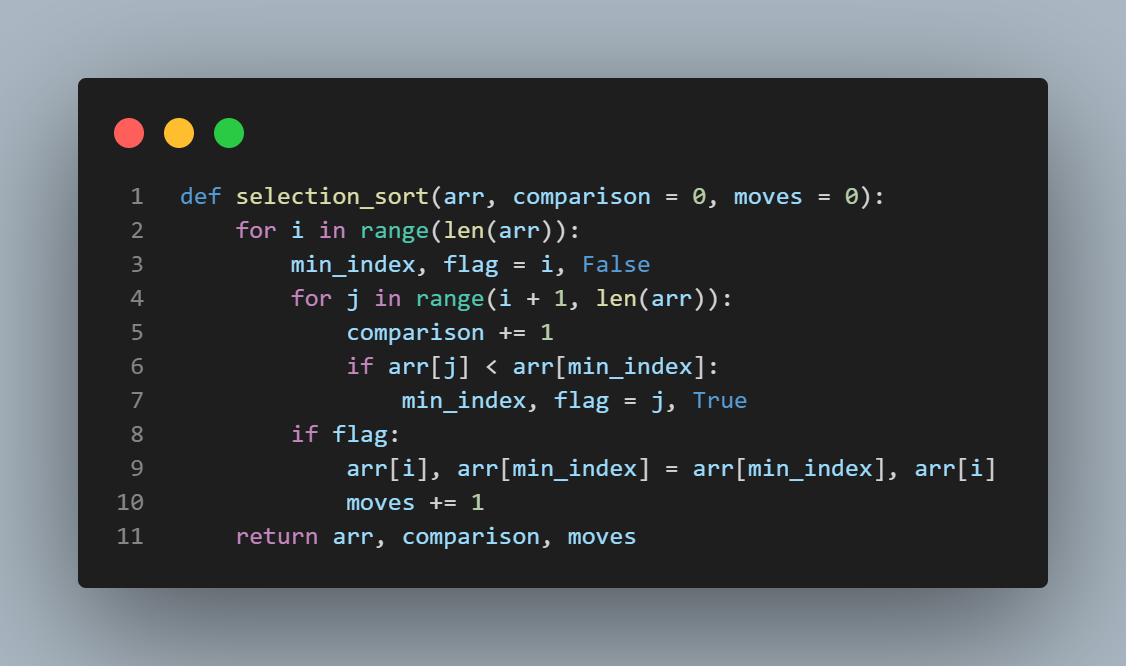
\includegraphics[width=1\linewidth]{Prt sc/Figure_1.png}  
        \end{minipage}
    \end{figure} \\
    Результати виконання алгоритму.
    \begin{figure}[h!]
        \begin{minipage}[h]{1\linewidth}
            \centering
            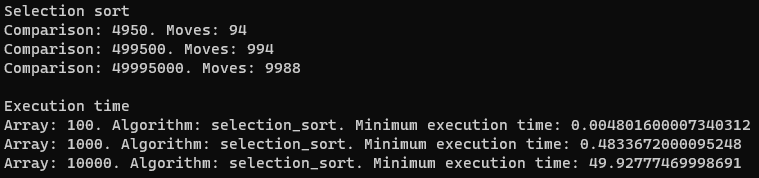
\includegraphics[width=1\linewidth]{Prt sc/Figure_2.png}
        \end{minipage}
    \end{figure}

\newpage
    \begin{center}
        \Large{Task \RomanNumeralCaps{2}}
    \end{center}
    \textbf{Написати програму, що реалізує метод швидкого соpтування.} \\
    $\sim n\log_2n$ 
    \begin{figure}[h!]
        \begin{minipage}[h]{1\linewidth}
            \centering
            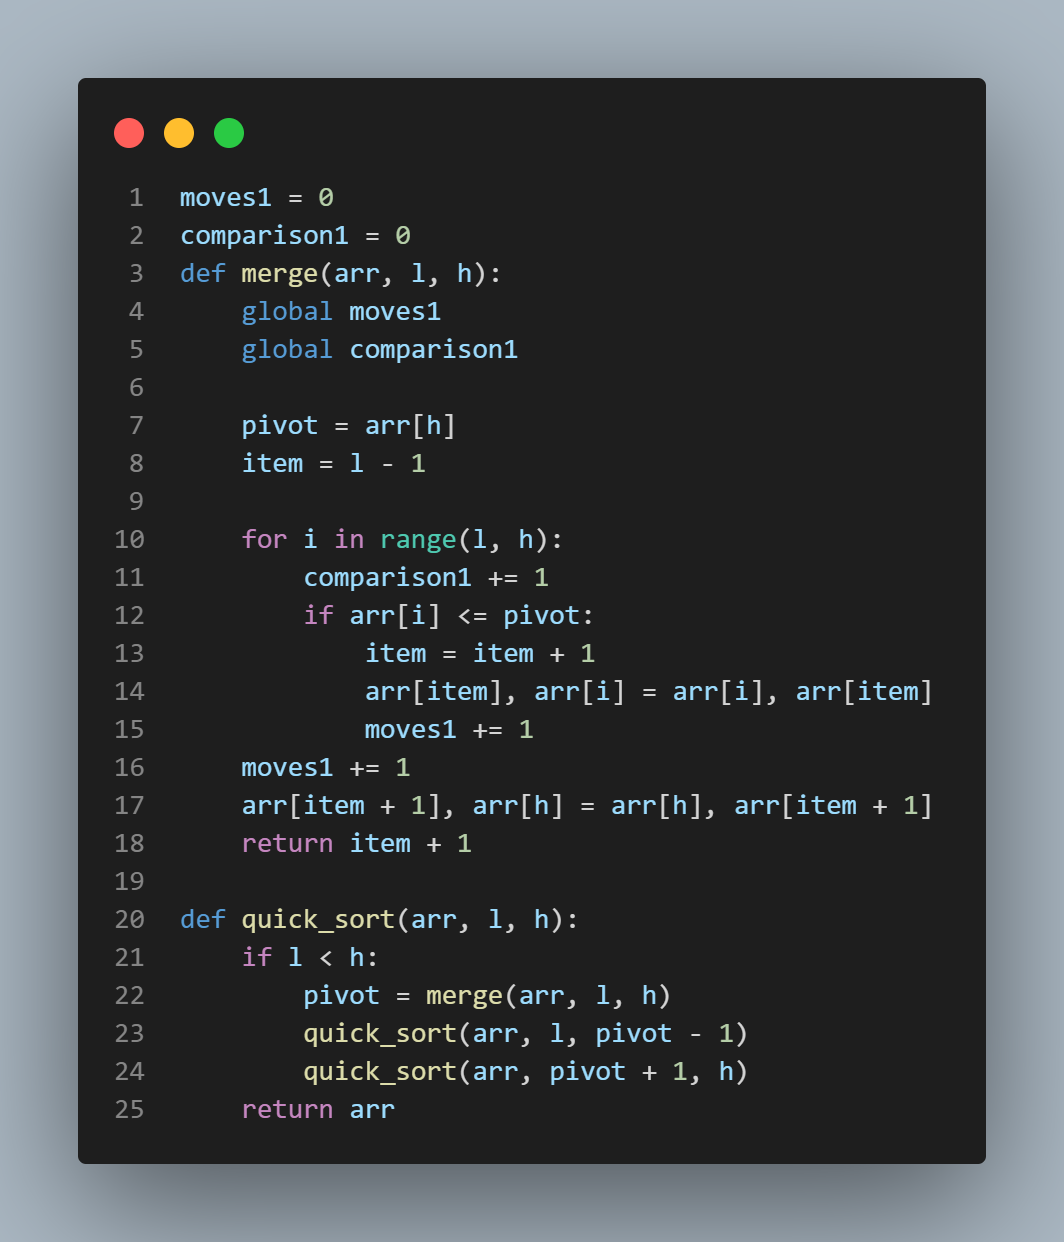
\includegraphics[width=0.9\linewidth]{Prt sc/Figure_3.png}  
        \end{minipage}
    \end{figure} \\
    Результати виконання алгоритму.
    \begin{figure}[h!]
        \begin{minipage}[h]{1\linewidth}
            \centering
            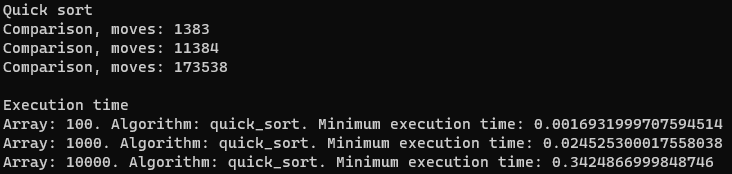
\includegraphics[width=1\linewidth]{Prt sc/Figure_4.png}
        \end{minipage}
    \end{figure}

\newpage
    Функція, що використовується для підрахунку часу виконання іншого блоку кода.
    \begin{figure}[h!]
        \begin{minipage}[h]{1\linewidth}
            \centering
            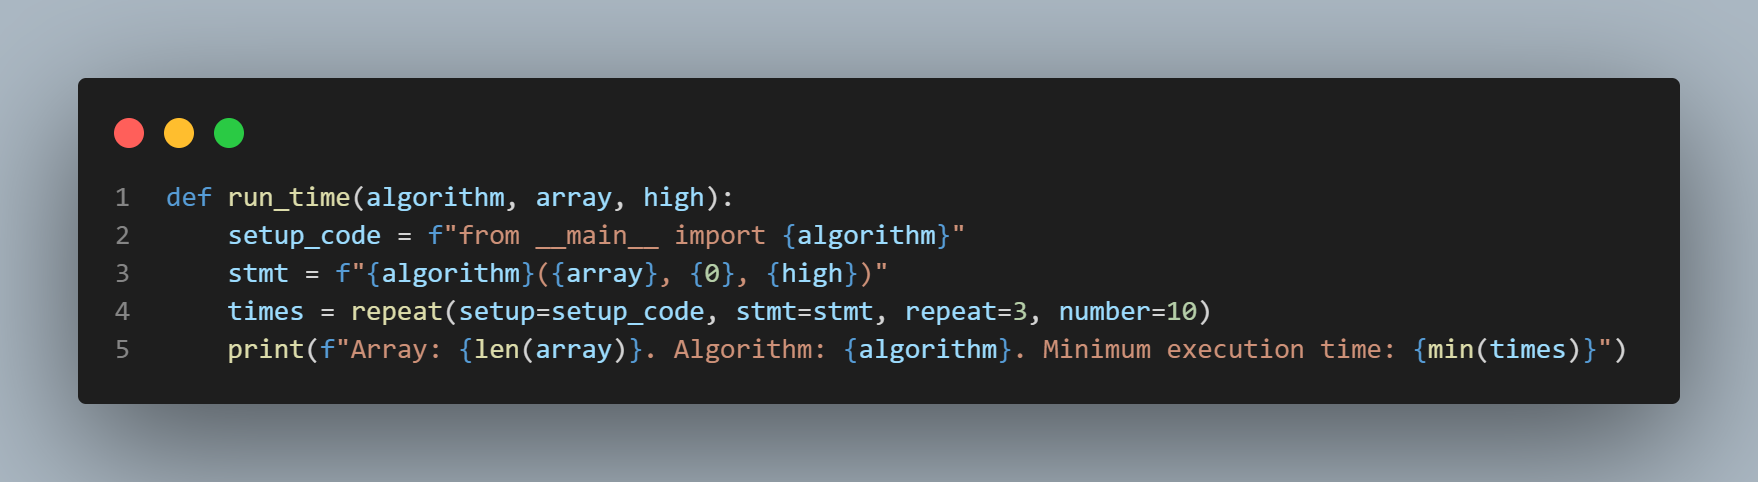
\includegraphics[width=1\linewidth]{Prt sc/Figure_5.png}
        \end{minipage}
    \end{figure} \\
    Початковий та відсортовані масиви.
    \begin{figure}[h!]
        \begin{minipage}[h]{1\linewidth}
            \centering
            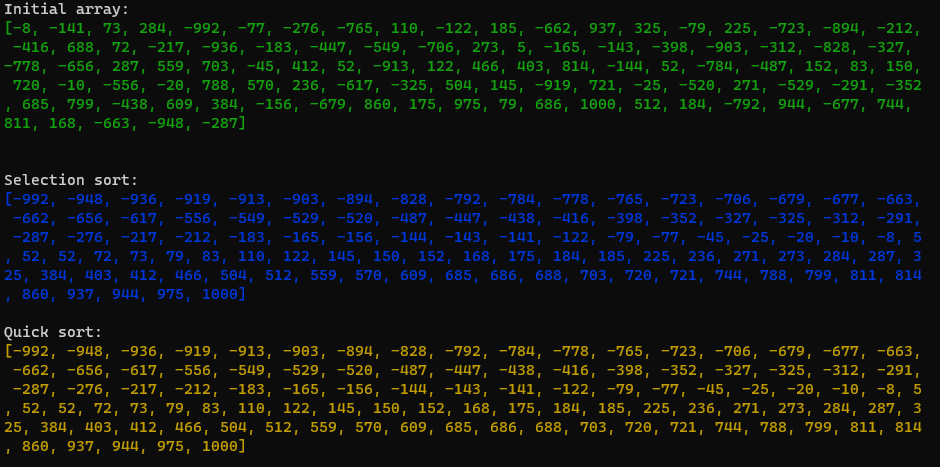
\includegraphics[width=1\linewidth]{Prt sc/Figure_6.png}
        \end{minipage}
    \end{figure}

\newpage
\KOMAoptions{paper=A4,paper=landscape,DIV=20,pagesize}
    \begin{center}
        \Large{Результати порiвняння методiв сортування}
    \end{center}
    
    \begin{table}[h]
        \centering
        \begin{tabular}{|c|ccccc|ccccc|}
            \hline
            &
            \multicolumn{5}{c|}{Сортування методом вибору} &
            \multicolumn{5}{c|}{Швидке сортування} \\ \hline
            \multirow{2}{*}{N} &
            \multicolumn{2}{c|}{\begin{tabular}[c]{@{}c@{}}К-ть копіювань\\ \\ (M)\end{tabular}} &
            \multicolumn{2}{c|}{\begin{tabular}[c]{@{}c@{}}К-ть порівнянь\\ \\ (C)\end{tabular}} &
            \multirow{2}{*}{\begin{tabular}[c]{@{}c@{}}Час\\ \\ (T)\end{tabular}} &
            \multicolumn{2}{c|}{\begin{tabular}[c]{@{}c@{}}К-ть копіювань\\ \\ (M)\end{tabular}} &
            \multicolumn{2}{c|}{\begin{tabular}[c]{@{}c@{}}К-ть порівнянь\\ \\ (C)\end{tabular}} &
            \multirow{2}{*}{\begin{tabular}[c]{@{}c@{}}Час\\ \\ (T)\end{tabular}} \\ \cline{2-5} \cline{7-10}
            &
            \multicolumn{1}{c|}{Теорет.} &
            \multicolumn{1}{c|}{Експерим.} &
            \multicolumn{1}{c|}{Теорет.} &
            \multicolumn{1}{c|}{Експерим.} &
            &
            \multicolumn{1}{c|}{Теорет.} &
            \multicolumn{1}{c|}{Експерим.} &
            \multicolumn{1}{c|}{Теорет.} &
            \multicolumn{1}{c|}{Експерим.} &
            \\ \hline
            100 &
            \multicolumn{1}{c|}{99} &
            \multicolumn{1}{c|}{93} &
            \multicolumn{1}{c|}{4950} &
            \multicolumn{1}{c|}{4950} &
            0.0047 &
            \multicolumn{1}{c|}{664} &
            \multicolumn{1}{c|}{688} &
            \multicolumn{1}{c|}{664} &
            \multicolumn{1}{c|}{1162} &
            0.001176 \\ \hline
            1000 &
            \multicolumn{1}{c|}{999} &
            \multicolumn{1}{c|}{996} &
            \multicolumn{1}{c|}{499500} &
            \multicolumn{1}{c|}{499500} &
            0.4166 &
            \multicolumn{1}{c|}{9966} &
            \multicolumn{1}{c|}{6285} &
            \multicolumn{1}{c|}{9966} &
            \multicolumn{1}{c|}{10955} &
            0.000992 \\ \hline
            10000 &
            \multicolumn{1}{c|}{9999} &
            \multicolumn{1}{c|}{9992} &
            \multicolumn{1}{c|}{49995000} &
            \multicolumn{1}{c|}{49995000} &
            43.4776 &
            \multicolumn{1}{c|}{132877} &
            \multicolumn{1}{c|}{81816} &
            \multicolumn{1}{c|}{132877} &
            \multicolumn{1}{c|}{159857} &
            0.2304 \\ \hline
        \end{tabular}
    \end{table}

\end{document}